\clearpage\section{CÀI ĐẶT VÀ KIỂM CHỨNG CHƯƠNG TRÌNH}
\subsection{Kiến trúc và luồng xử lý}
Kiến trúc phần mềm gồm các thành phần dữ liệu, nguy cơ, tối ưu, kiểm chứng và trực quan hóa. Bộ sinh A4 thiết lập đồ thị; mô-đun nguy cơ xác định các mốc đóng; bộ giải và bộ kiểm tra lần lượt tạo lịch và đánh giá tính khả thi. Thành phần trực quan hóa đọc kết quả đã lưu.

\begin{figure}[htbp]\centering
\begin{tikzpicture}[>=Stealth,every node/.style={font=\footnotesize,draw,rounded corners,align=center,minimum width=2.1cm,minimum height=1.1cm},node distance=.45cm]
\node (a) {Mặt bằng\\và tham số};
\node[right=of a] (b) {Đồ thị\\và nguy cơ};
\node[right=of b] (c) {Bộ giải\\M1--M4};
\node[right=of c] (d) {Lịch và\\kiểm chứng};
\node[right=of d] (e) {Chỉ số và\\phát lại};
\draw[->] (a)--(b);\draw[->] (b)--(c);\draw[->] (c)--(d);\draw[->] (d)--(e);
\end{tikzpicture}\caption{Luồng dữ liệu của chương trình CLI.}\end{figure}

\begin{table}[htbp]\centering\caption{Các mô-đun chính}
\small\begin{tabularx}{\linewidth}{P{4.5cm}X}\toprule
Tệp & Trách nhiệm\\\midrule
\texttt{data.py}, \texttt{hazards.py} & Nhập sơ đồ, lưu giả định, tính mốc nguy cơ.\\
\texttt{algorithms.py} & Dijkstra, đa nguồn, Dinic, Min-Cost Flow tự viết.\\
\texttt{optimize.py}, \texttt{baselines.py} & TEN, M4 và ba bộ đối chứng.\\
\texttt{schedule.py}, \texttt{runner.py} & Kiểm tra, phát lại, đo và xuất dữ liệu.\\
\texttt{visuals.py}, \texttt{cli.py} & Hiển thị và giao diện dòng lệnh.\\\bottomrule
\end{tabularx}\end{table}
Các thuật toán chính được cài đặt trong mô-đun nội bộ. NetworkX chỉ đóng vai trò tham chiếu trong kiểm thử đồ thị nhỏ.

\topic{Cấu trúc dữ liệu và hợp đồng đầu vào}
Các cấu trúc Node và Edge lưu thông tin đủ để solver và bộ phát lại cùng hiểu một hành động. Node có ID, tầng, tọa độ, loại, sức chứa, quyền chờ và năng lực thoát. Edge có hai đầu, chiều dài, thời gian, năng lực vào, sức chứa đang đi và loại cạnh. Mọi ID được lập chỉ mục để phát hiện trùng và tra cứu nhất quán.

\begin{lstlisting}
Node(id, floor, x, y, kind,
     storage_capacity, can_wait, exit_capacity)
Edge(id, source, target, length_m,
     travel_seconds, entry_capacity,
     in_transit_capacity, kind)
Action(kind, source, target, depart,
       arrive, edge_id)
Journey(id, source, count, actions,
        exit_node, exit_step)
\end{lstlisting}
Ràng buộc kiểu dữ liệu yêu cầu dân số là số nguyên không âm, không vượt sức chứa khu phòng và loại trừ kiểu logic. Các tham số thời gian, tốc độ phải hữu hạn và thuộc miền hợp lệ. Đặc trưng hình học được quản lý riêng với tham số động lực học để duy trì ngữ nghĩa của từng trường cấu hình.

Kiểm tra cấu trúc bảo đảm các đầu cạnh tồn tại, chiều dài và thời lượng dương, EXIT có tính hấp thụ và liên kết giữa tầng chỉ xuất hiện tại các nút thang. Các cấu hình sức chứa không được biểu diễn đầy đủ bởi mô hình đoàn bị loại khỏi miền đầu vào hợp lệ.

Mỗi lượt thực nghiệm lưu mô hình trong \texttt{building.json}, phân bố dân số trong \texttt{occupancy.json}, kịch bản trong \texttt{scenario.json} và tập giả định trong tệp riêng. Định danh cấu trúc mạng và mã băm đầu vào phục vụ truy xuất cấu hình, đối chiếu các phương pháp và kiểm soát việc tái sử dụng kết quả.

\topic{Thứ tự sự kiện, phát lại và bảo toàn dân số}
Tại mỗi mốc, chương trình xét các người vừa đến, kiểm tra tồn tại tại nút, thực hiện lệnh rời và ghi nhận thoát. Sức chứa nút được đo sau đến nhưng trước rời; trace còn lưu thêm số tại nút sau rời để cộng với người đang đi. Hai đại lượng này có mục đích khác nhau, không thay thế tùy ý khi kiểm tra.

\begin{equation}N=N_{node}(k)+N_{move}(k)+N_{exit}(k)+N_{exposed}(k).\end{equation}
Trong đó $N_{node}$ là số tại nút sau khởi hành, $N_{move}$ là số còn trên cạnh, $N_{exit}$ là số thoát tích lũy và $N_{exposed}$ là số chưa thoát đang ở vị trí mất an toàn. Phần dân số chưa được sơ tán luôn được bảo toàn trong hệ thống thống kê, bao gồm trạng thái mắc kẹt hoặc phơi nhiễm.

\begin{table}[htbp]\centering\caption{Ví dụ phát lại 20 người ở phòng 101, bước 5 s}
\small\begin{tabular}{rrrrr}\toprule Mốc (s) & Trong phòng & Đang đi & Đã thoát & Tổng\\\midrule
0 & 13 & 7 & 0 & 20\\
5 & 6 & 7 & 7 & 20\\
10 & 0 & 6 & 14 & 20\\
15 & 0 & 0 & 20 & 20\\\bottomrule\end{tabular}\end{table}
Ví dụ dùng cửa có năng lực bảy người/bước và cạnh phòng--cửa mất một bước. Ba đoàn đi 7, 7, 6; sự kiện thoát trùng mốc đến cửa. Không có một đoàn nào phải chờ một cổng giả định sau cửa phòng.

Bộ kiểm tra tái dựng mức sử dụng tài nguyên từ hành động và đánh giá tính liên tục nguồn--đích, mốc đi/đến, thời lượng cạnh, năng lực vào, lượng đang đi, sức chứa nút và mốc nguy hiểm. Kết luận khả thi được xác lập từ dữ liệu lịch; các chỉ số tổng hợp lưu trước không thay thế bước kiểm chứng này.

\topic{Thiết kế kiểm thử và đối chứng thuật toán}
Bộ kiểm thử gồm 48 ca đạt yêu cầu, tập trung vào kết quả chuẩn, ranh giới thời gian và lỗi biến đổi lịch. Các ca tham số hóa theo seed kiểm tra những đồ thị nhỏ có nghiệm đối chứng; chúng tách biệt với thực nghiệm A4.

\begin{table}[htbp]\centering\caption{Nhóm kiểm thử và lỗi cần phát hiện}
\small\begin{tabularx}{\linewidth}{P{4.2cm}X}\toprule
Nhóm & Mục tiêu\\\midrule
Đường đi, đa nguồn & Trọng số 0, A*, không có đường, nhiều thời điểm nguồn.\\
Luồng và chi phí & 25 seed đồ thị nhỏ so với NetworkX; cạnh dư sửa lựa chọn cũ.\\
Độ sâu mạng & Chuỗi 2.100 cạnh không lỗi đệ quy.\\
Nhập A4 & Tổng 1.360, 27 khu, 50 cửa, thứ tự phòng và bỏ WC.\\
Hành lang hở & Đến cửa là thoát; cửa vẫn là nút thắt; thang bị chặn không chặn mọi phòng tầng 1.\\
Lịch và trace & Bảo toàn dân số, biên nguy hiểm, lịch rỗng/thiếu và dữ liệu bị sửa.\\
Tái sử dụng & Từ chối cache khác topology dù cùng tham số.\\\bottomrule
\end{tabularx}\end{table}

Bộ đối chứng sử dụng hai hàm của NetworkX \cite{networkx}:
\begin{itemize}
\item \texttt{maximum\_flow\_value}: xác định giá trị luồng cực đại.
\item \texttt{max\_flow\_min\_cost}: xác định luồng cực đại có tổng chi phí nhỏ nhất.
\end{itemize}
Kiểm thử so sánh giá trị luồng và chi phí nghiệm trên cùng đồ thị nguyên.

Kiểm chứng gồm các lớp bổ sung: lập luận về bất biến thuật toán, đối chiếu với bộ giải tham chiếu, kiểm thử ranh giới và phát lại lịch. Cách kết hợp này bao phủ cả sai sót giải thuật lẫn sai sót ánh xạ metadata, điều kiện biên và thống kê trạng thái sau tối ưu.

\topic{Quy trình thực nghiệm và khả năng tái lập}
Mỗi lượt được nhận diện bằng phiên bản dữ liệu, cấu trúc mạng, phân bố dân số, kịch bản và seed. Các lệnh dưới đây chạy thực nghiệm và kiểm tra lịch từ gói mã nguồn \cite{code}; hướng dẫn cài đặt và biên dịch nằm trong README.

\begin{lstlisting}[language={},caption={Các bước chạy thực nghiệm và kiểm tra lịch}]
$results = "outputs/a4_open_ground/benchmark"
python -m pytest -q
python -m a4_evac generate-data
python -m a4_evac benchmark --output $results
python -m a4_evac replay "$results/safe/M4"
\end{lstlisting}
Lịch, trạng thái, nguy cơ, hàng đợi và chỉ số được lưu cùng kết luận kiểm tra. Kết quả chỉ được tái sử dụng khi đầu vào trùng khớp và lịch đạt kiểm tra lại. Thời gian giải được đo quanh lời gọi solver, tách khỏi dựng hình và ghi tệp. Công cụ tracemalloc \cite{tracemalloc} chỉ theo dõi cấp phát Python; lượt không bật đo bộ nhớ được lưu giá trị thiếu.

\topic{Trực quan hóa lịch và thang thời gian trình chiếu}
GIF phát lịch đã kiểm chứng, lấy mẫu mỗi 5 s và hiển thị 600 ms/khung. Tốc độ trình chiếu độc lập với thời lượng hành động. Hình dưới tổng hợp năm khung theo tầng để đọc được số người; kiểm tra sức chứa và an toàn vẫn dùng bản ghi sự kiện chi tiết.

\begin{figure}[htbp]\centering
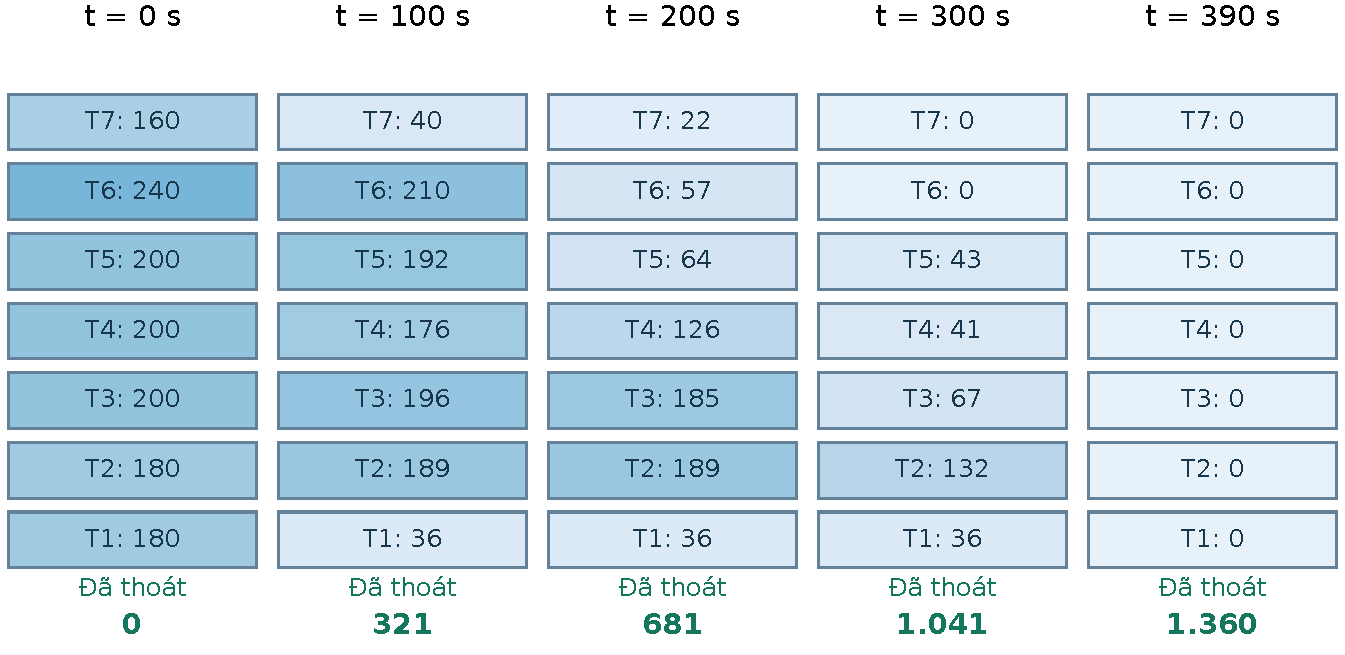
\includegraphics[width=\linewidth]{figures/timeline.pdf}
\caption{Năm khung phát lại giản lược theo tầng của lịch M4 tại 0, 100, 200, 300 và 390 s. Mỗi ô ghi số người còn trong hệ tại một tầng; người đang đi được quy về tầng đầu cạnh. Dòng xanh ghi số đã thoát. Tổng mỗi khung luôn bằng 1.360.}
\label{fig:timeline}\end{figure}
